\documentclass[11pt]{aastex}
\usepackage{geometry}                % See geometry.pdf to learn the layout options. There are lots.
\geometry{letterpaper}                   % ... or a4paper or a5paper or ... 
%\geometry{landscape}                % Activate for for rotated page geometry
%\usepackage[parfill]{parskip}    % Activate to begin paragraphs with an empty line rather than an indent
\usepackage{graphicx}
\usepackage{amssymb}
\usepackage{epstopdf}
\DeclareGraphicsRule{.tif}{png}{.png}{`convert #1 `dirname #1`/`basename #1 .tif`.png}

\title{A Relation between Mass and Radius for 59 Exoplanets with $\rpl <  \rspecial$}
\author{L. M. Weiss \& G. W. Marcy}
%\date{}                                           % Activate to display a given date or no date

%---------------------------- Physical Quantities ------------------------------------%
\newcommand{\kms}{\ensuremath{\rm km\,s^{-1}}}
\newcommand{\ms}{\ensuremath{\rm m\,s^{-1}}}
\newcommand{\mse}{\ensuremath{\rm m\,s^{-1}}}
\newcommand{\gcmc}{\ensuremath{\rm g\,cm^{-3}}}
\newcommand{\gcc}{\gcmc}
\newcommand{\fluxunit}{\ensuremath{\rm erg\,s^{-1}\,cm^{-2}}}
\newcommand{\rhk}{\ensuremath{R^{\prime}_{\rm HK}}}	% Activity index R'_HK
\newcommand{\logrhk}{\ensuremath{\log\rhk}}		% log of R'_HK

\newcommand{\teff}{\ensuremath{T_{\rm eff}}}
\newcommand{\logg}{\ensuremath{\log{g}}}
\newcommand{\vsini}{\ensuremath{v \sin{i}}}
\newcommand{\feh}{[Fe/H]}
\newcommand{\logl}{\ensuremath{\log{L}}}

\newcommand{\rsun}{\ensuremath{R_\sun}}
\newcommand{\msun}{\ensuremath{M_\sun}}
\newcommand{\lsun}{\ensuremath{L_\sun}}

\newcommand{\rstar}{\ensuremath{R_\star}}
\newcommand{\mstar}{\ensuremath{M_\star}}
\newcommand{\loggstar}{\ensuremath{\logg_\star}}
\newcommand{\lstar}{\ensuremath{L_\star}}
\newcommand{\astar}{\ensuremath{a_\star}}
\newcommand{\loglstar}{\ensuremath{\log{L_\star}}}
\newcommand{\rhostar}{\ensuremath{\rho_\star}}

\newcommand{\rpl}{\ensuremath{R_{\rm P}}}
\newcommand{\mpl}{\ensuremath{M_{\rm P}}}
\newcommand{\lpl}{\ensuremath{L_{\rm P}}}
\newcommand{\rhopl}{\ensuremath{\rho_{\rm P}}}
\newcommand{\loggpl}{\ensuremath{\logg_{\rm P}}}
\newcommand{\teq}{\ensuremath{T_{\rm eq}}}

\newcommand{\rjup}{\ensuremath{R_{\rm J}}}
\newcommand{\mjup}{\ensuremath{M_{\rm J}}}
\newcommand{\rhojup}{\ensuremath{\rho_{\rm J}}}
\newcommand{\rearth}{\ensuremath{R_\earth}}
\newcommand{\mearth}{\ensuremath{M_\earth}}
\newcommand{\fearth}{\ensuremath{F_\earth}}

\newcommand{\msini}{\ensuremath{m \sin{i}}}
\newcommand{\mplsini}{\ensuremath{\mpl\sin{i}}}

\newcommand{\npl}{226~} % The number of exoplanets used to determine the MRF relation
\newcommand{\nhires}{42~} % The number of transiting planets in the HIRES paper
\newcommand{\nlm}{59~}
\newcommand{\rspecial}{4 \rearth}
\newcommand{\chisquared}{3.4~}
\newcommand{\chiquad}{6.5~}
\newcommand{\rms}{3.8 \mearth}

\begin{document}
\maketitle
%\begin{abstract}
We study the masses and radii of the 59 known exoplanets that have radii less than 4\rearth.  We find a linear relation of the form $\mpl \approx 3\rpl$.  The RMS of planet masses is \rms, and our best fit has reduced $\chi^2=\chisquared$, indicating a large diversity in planet compositions below 4\rearth.  \citet{WL2013}, who also find $\mpl \approx 3\rpl$, note that the linear scaling is consistent with a constant escape velocity.
%\end{abstract}

\section{Introduction}
%\subsection{}

The Kepler Mission has found an abundance of planets with  $R < 4 \rearth$ \citep{Batalha2012}.  However, in many systems, it is difficult to measure the masses of such small planets because the gravitational acceleration these planets induce on their host stars or neighboring planets is too small to detect with current telescopes and instruments.  How can we determine the composition of these planets?

\citet{Weiss2013} have shown that for planets between a few and thousands of Earth masses, we can predict the radius of a planet from its mass and incident stellar flux, suggesting that planets of a given mass have a particular composition.  However, below $\sim$4 \rearth, the large apparent scatter in planet mass makes predicting planet mass harder.  At 2 \rearth, planets are observed to span a decade in densities, from less dense than water to densities suggesting a solid iron composition.

There are two explanations for the large apparent scatter in planet densities: either errors in radius and/or mass measurements are underestimated for planets below 4 \rearth, or the (real) scatter in radius indicates a diversity of planet compositions.   Identifying whether this apparent variety in planet densities is real or not is one of the most pressing issues in understanding planetary compositions today.  Does the size of a planet uniquely determine a planet's composition, or is there diversity of the rock, water, and H/He composition at a given mass?  If the scatter is only apparent, then it is possible that there is a one-to-one correspondence between planet size and composition below 4 \rearth.  However, if the scatter is real, then there must be a diversity of planet compositions at a given mass below 4 \rearth.  Further refinements to the measurements of planet masses, especially below 4 \rearth, are necessary to test to what extent the apparent scatter of planetary masses at a given radius is real.

Another way to probe the scatter in planet mass is to attempt to measure the masses of more small planets.  Although uncertainties in the mass measurements for individual planets might be of order the planet mass, observing many small planets allows us to study the statistical distribution of planet masses for small planets.  \citet{Marcy2013} have taken this approach to measure the masses of 42 small, transiting planets.  This wealth of new data merits a reconsideration of the relation between planet mass and radius for small planets, which is the subject of this paper.

This updated examination of the mass-radius relation benefits from the masses and radii of \npl expo planets with $\rpl < \rspecial$.  The sources of these measurements are (1) the masses of \nhires planets with $\rpl < \rspecial$ from 22 stellar systems, characterized in \citet{Marcy2013}, and (2) additional planets and/or refined stellar parameters for several systems, including 55 Cnc e \citep{Endl2012}?, Kepler-11 \citep{Lissauer2013}, GJ 3470 \citep{Demory2013}, HD 97658 b \citep{Dragomir2013}, and KIC 8435766 \citep{Sanchis-Ojeda2013}

A plot of radius versus mass for \npl exoplanets is shown in Figure \ref{fig:mrf}.  The planets are colored by incident flux from the host star; planets that receive more than the median flux (459 Earth fluxes) are red, while those that receive less are blue.  Most of the planets that have been discovered since the publication of \citet{Weiss2013} are in the low-mass branch of this diagram.  For this reason, and also because the relation between mass and radius for small planets is both poorly understood and vital for determining planet composition of small planets, we focus on the low-mass portion of the population.  In the rest of this paper, we examine planets for which $\rpl < \rspecial$.  We try to determine how their size correlates with their masses and densities (and therefore compositions), and we also investigate how other parameters might correlate with the physical properties of these small exoplanets.

\section{Using Negative Planet Masses for Statistical Soundness}
\citet{Marcy2013} allow ``negative" planet masses as Keplerian orbital solutions to avoid the Lutz-Kelker bias.  A ``negative" planet mass arises when, given the orbital period and phase determined by the transit, the RV data have the opposite sign from what is expected.  This yields a negative semi-amplitude $K$ in the orbital solution, which results in a negative planet mass.  See \citet{Marcy2013} for a more detailed discussion of this technique.
 
In a traditional analysis, the uncertainties in the RVs and the number of measurements combine to determine an upper limit to the planet mass.  However, upper limits to planet masses are difficult to use statistically.  The artifice of a negative planet mass allows us to treat the population of small planets statistically.  Since there is no bias toward large or small planet masses in our sample, we can take the weighted mean mass of planets of a given radius.

\section{Justification for a Mass-Radius Relation for Small Exoplanets}
Is there a correlation between planet mass and radius for small ($\rpl < \rspecial$) exoplanets?  By eye, we might judge that there is a correlation, but what is the probability that we have fooled ourselves into believing there is a correlation when there is none?

To answer this question, we calculate the probability that mass and radius are uncorrelated.  First, we calculate the correlation coefficient (Pearson R test) $r=0.61$ .  There are 59 planets smaller than 4 \rearth, leaving 57 degrees of freedom, so the Student t value is 5.75.  The probability that these data are uncorrelated is $1.3 \times 10^{-6}$.  Thus, the masses and radii of planets between the sizes of Earth and Neptune are correlated.

Another way to convince yourself that mass and radius are correlated for small planets is to examine Figure \ref{fig:rbin}, which shows the weighted mean exoplanet mass in bins of width 1 \rearth.  On average, exoplanet mass increases with increasing radius, indicating an underlying correlation in the individual exoplanet masses and radii.

We conclude that for $\rpl < 4 \rearth$, exoplanet mass increases with increasing exoplanet radius.

\section{The Updated Mass-Radius Relation for Small Exoplanets}
Figure \ref{fig:rm_4} suggests that exoplanet masses and radii can be fit with a line.  We verify this with a traditional power-law fit and obtain $\mpl \propto \rpl$ as the best result.

The best linear fit to the data for $\rpl < \rspecial$ is:
$$
\mpl/\mearth = 0.2  +     2.6~\rpl/\rearth
$$
There are 59 exoplanets in this sample.  The reduced $\chi^2=\chisquared$, and the RMS $=\rms$.

To illustrate how this population of exoplanets compares to our Solar System, we plot the Solar System planets in Figure \ref{fig:rm_4} as blue triangles.  A quadratic fit to the exoplanet population happens to line up with the Solar System planets, but has a reduced $\chi^2$ that is twice as large as the linear fit to the exoplanets.  Since most of the exoplanets in this sample have $P < 50$ days, we do not expect them to behave the same way as Uranus and Neptune, which have orbital periods of tens of thousands of days.  Therefore, the hefty masses of Uranus and Neptune compared to planets of similar size that are closer to their stars is not unreasonable.  In fact, the difference in mass between Uranus and Neptune compared to closer-in planets of 4 \rearth\ distinguishes the quadratic fit as good for the solar system, as compared to the linear fit that is good for exoplanets.

\section{Discussion}
	
\subsection{Interpretation of the Mass-Radius Relation}
The correlation between exoplanet mass and radius for $\rpl < 4 \rearth$ indicates that Earth-size planets are less massive than Neptune-size planets.

The large reduced $\chi^2$ values for the linear and quadratic mass-radius relations indicate that these relations are not sufficient models to explain the variation in planet mass at a given radius.  Either a diversity of planet compositions, or correlation between the residuals and some other parameter, is required to explain the large scatter in planet mass.

The data are better described by a linear fit than a quadratic or cubic fit.  Since a cubic fit of $\mpl \propto \rpl^3$ describes how mass and radius relate for constant density, a fit of $\mpl \propto \rpl$ indicates that planet density decreases strongly as mass or radius increases (see Figure \ref{fig:rbin} and \ref{fig:rhor}).  This can be attributed to an increasing fraction of volatiles with increasing planet mass.

Previous work, including \citet{Lissauer2011} and \citet{Weiss2013}, suggest that the mass-radius relation is more like $\mpl \propto \rpl^2$ for small exoplanets.  However, these studies include Saturn or Saturn-like planets at the high-mass end of their populations.  Such planets might better be described as part of the giant planet population.  Using the properties of Saturn-like planets in a relation that attempts to describe the properties of planets that are more like Earth and Neptune is misleading.  

In a study of planets with $\mpl < \sim20\mearth$, \citet{WL2013} found $\mpl/\mearth \approx 3 \rpl/\rearth$ in a sample of 22 pairs of planets that exhibited strong anti-correlated transit timing variations (TTVs).  Our independent assessment of 59 planets, 43 of which are newly reported and are not analyzed in \citet{WL2013}, agrees with this result.

\citet{WL2013} noted that a linear relation between planet mass and radius is dimensionally consistent with a constant escape velocity from the planet (i.e. $v_{\mathrm{esc}}^2 \sim \mpl/\rpl$).  While this is one interpretation of the linear mass-radius relation for small exoplanets, there are perhaps other valid physical interpretations.  For instance, a constant $\mpl/\rpl$ implies that the gravitational potential energy $U \propto \mpl/\rpl$ of exoplanets is constant.  This could be due to atmospheric particles escaping, but perhaps some other physical mechanism sets this energy level for exoplanets.

\subsection{The Possible Role of Photoevaporation in Sculpting Small Planets}
Strong stellar irradiation can either inflate a planet, as with hot Jupiters \citep{Seager2007}, or it can photoionize and strip the planet's atmosphere, leaving a dense core \citep{Lopez2012}.  Possible evidence for these processes can be seen in Figure \ref{fig:flux_radius}, which shows that for massive planets ($\mpl > 60 \mearth $ or $\rpl > \rspecial$), high incident flux correlates with larger radius, whereas for low-mass planets ($\mpl < 60 \mearth $ or $\rpl < \rspecial$), high incident flux correlates with smaller radius.

Another way to describe how incident flux relates to exoplanet size is that for low levels of incident stellar flux (less than 100 times what Earth receives), you can find planets ranging in size from Earth to Jupiter.  However, at higher incident flux, there are only hot Earths (which might have been photo-evaporated) and hot Jupiters (which have been inflated).  In other words, there are no hot Neptunes.  Given the detection of hot and cold Earths, hot and cold Jupiters, and cold Neptunes, it seems unlikely that a detection bias causes the dearth of hot Neptunes; rather, their absence is likely astrophysical.

How significant is the decrease in planet size with increasing planet flux for small exoplanets?  For $\rpl < \rspecial$, we find a correlation Pearson R coefficient between planet radius and incident stellar flux of $r=-0.19$.  Over a sample of 71 planets, this corresponds to a Student-t value of $t=-1.6$, indicating a probability of 0.11 that these variables are uncorrelated.  Repeating this calculation for a larger sample of exoplanets (for instance, the entire catalog of Kepler planets candidates, for which \rpl and the incident flux on the planet are known) would reveal whether this correlation is real.

\begin{comment}
\subsection{Do Small Planets form around Small Stars?}
Although several studies find that planet radius correlates with stellar mass, we find no correlation in this sample (Pearson R = 0.05).  This is partly because our planets are smaller than $4 \rearth$.  However, some planets in our sample have $4 \rearth < \rpl < 7 \rearth$, in which range \citet{WL2013} find a correlation between planet size and stellar mass. 
\end{comment}

\subsection{Correlation with Residuals}
We examine the possibility that the residuals to the mass-radius fit correlate with some other parameter.  The correlation between the residual (exoplanet mass minus predicted mass) and each of: the incident flux from the star, the semi-major axis, the orbital period, the stellar mass, and the stellar radius, all had magnitudes less than 0.1.  The residuals as a function of orbital period, semi-major axis, and incident flux are shown in figure \ref{fig:mr_residuals}.  For all of the parameters listed above, the probability that the residuals do not correlate with each parameter is at least $ 0.3$ (i.e. mass residuals have at most a probability of 0.7 of correlating with one of the parameters listed above).

\subsection{Interpretation of Planet Compositions}
For detailed models of the compositions of the 42 new transiting planets presented in \citet{Marcy2013} and analyzed here, see \citet{Rogers2013}.  Here, we consider the statistical properties of planet densities.

The densities of exoplanets with $\rpl < \rspecial$ are shown in Figure \ref{fig:rhor}, and the densities binned by 1 \rearth are shown in Figure \ref{fig:rbin}.  Although the individual measurements of density for planets with $\rpl < 2 \rearth$ have large uncertainties (Figure \ref{fig:rhor}), the weighted mean densities (Figure \ref{fig:rbin}) for 0-1 \rearth and 1-2 \rearth show the continuation of the trend that smaller planets have higher densities.  Figure \ref{fig:rhor} shows a dashed line at the density of Earth.  Planets smaller than 2 \rearth tend to be denser than Earth, whereas planets larger than 2 \rearth tend to be less dense than Earth.  However, since rock and other materials are compressible, planets that are as dense as Earth but have larger radii are not necessarily solid rock; they need some lighter materials, such as water or a H/He envelope, to achieve the density of Earth.

\section{Conclusions}
For exoplanets with $\rpl < \rspecial$ and $P < ~\sim100$ days, planet radius correlates with planet mass.  In this regime, the scaling between planet mass and radius is linear: $\mpl/\mearth \approx 3\rpl/\rearth$, indicating that larger planets have substantially more volatiles than smaller planets.  This relation is also different than what we observe for the Solar System planets smaller than Saturn, since Uranus and Neptune are more massive than the exoplanets of their size in this sample.  A study of exoplanets of 3-4 \rearth with orbital periods of dozens of years would better contextualize Uranus and Neptune.

One reason Uranus and Neptune might be more massive than closer-in planets of the same size is that incident stellar flux might photo evaporate the atmospheres of closer-in counterparts, causing mass loss.  The correlations between planet size and incident flux from the star for both large and small planets, and the absence of hot Neptunes, indicate that incident stellar flux of more than 100 times what Earth receives might play a key role in sculpting close-in planets.

%% The values (usually only l,r and c) in the last part of
%% \begin{deluxetable}{} command tell LaTeX how many columns
%% there are and how to align them.
\begin{deluxetable}{lllllll}

%% Keep a portrait orientation


%% Over-ride the default font size
%% Use 10pt
\tabletypesize{\tiny}

\tablewidth{0pt} %to over-ride the default table width.
%% If you are unhappy with the default look at the end of the
%% *.log file to see what the default was set at before adjusting
%% this value.

%% This is the title of the table.
\tablecaption{Exoplanets with Measured Mass and Radius and $\rpl < \rspecial$}
%% This command over-rides LaTeX's natural table count
%% and replaces it with this number.  LaTeX will increment 
%% all other tables after this table based on this number
\tablenum{1}
\label{tab:mrf}

%% The \tablehead gives provides the column headers.  It
%% is currently set up so that the column labels are on the
%% top line and the units surrounded by ()s are in the 
%% bottom line.  You may add more header information by writing
%% another line between these lines. For each column that requries
%% extra information be sure to include a \colhead{text} command
%% and remember to end any extra lines with \\ and include the 
%% correct number of &s.
\tablehead{\colhead{Name} & \colhead{Planet Mass} & \colhead{Planet Radius} & \colhead{Incident Flux} & \colhead{Period} & \colhead{First Ref.} & \colhead{Orbital Ref.} \\ 
\colhead{} & \colhead{($M_\earth$)} & \colhead{($R_\earth$)} & \colhead{($F_\earth$)} & \colhead{(d)} & \colhead{} & \colhead{} } 

%% All data must appear between the \startdata and \enddata commands
\startdata
            55 Cnc e &      8.380 &      2.210 &   2439.690 &      0.737 &                     \citet{McArthur2004} &                         \citet{Endl2012}\\ 
           CoRoT-7 b &      5.021 &      1.679 &   1779.433 &      0.854 &             \citet{Queloz2009,Leger2009} &                       \citet{Queloz2009}\\ 
           CoRoT-8 b &     68.673 &      6.389 &     88.184 &      6.212 &                        \citet{Borde2010} &                        \citet{Borde2010}\\ 
           GJ 1214 b &      6.260 &      2.800 &     16.631 &      1.580 &                  \citet{Charbonneau2009} &                       \citet{Carter2011}\\ 
           GJ 3470 b &     13.900 &      4.830 &     38.335 &      3.337 &                      \citet{Bonfils2012} &                      \citet{Demory2013}\\ 
            GJ 436 b &     23.105 &      4.222 &     29.882 &      2.644 &                       \citet{Butler2004} &                       \citet{Maness2007}\\ 
          HAT-P-11 b &     26.231 &      4.730 &     97.355 &      4.888 &                        \citet{Bakos2010} &                        \citet{Bakos2010}\\ 
          HAT-P-26 b &     18.640 &      6.333 &    163.050 &      4.235 &                     \citet{Hartman2011b} &                      \citet{Hartman2011b} \\ 
          HD 97658 b   &  7.862   &  2.340  &  48.052  &   9.491      &                \citet{Howard2011}        &            \citet{Dragomir2013}\\
         Kepler-10 b &      4.539 &      1.416 &   3572.048 &      0.837 &                      \citet{Batalha2011} &                      \citet{Batalha2011}\\ 
         Kepler-11 b &      1.900 &      1.800 &    126.384 &     10.304 &                     \citet{Lissauer2011} &                     \citet{Lissauer2013}\\ 
         Kepler-11 c &      2.900 &      2.870 &     91.413 &     13.025 &                     \citet{Lissauer2011} &                     \citet{Lissauer2011}\\ 
         Kepler-11 d &      7.300 &      3.120 &     43.562 &     22.687 &                     \citet{Lissauer2011} &                     \citet{Lissauer2011}\\ 
         Kepler-11 e &      8.000 &      4.190 &     27.524 &     31.996 &                     \citet{Lissauer2011} &                     \citet{Lissauer2011}\\ 
         Kepler-11 f &      2.000 &      2.490 &     16.745 &     46.689 &                     \citet{Lissauer2011} &                     \citet{Lissauer2011}\\ 
         Kepler-18 b &      6.900 &      2.000 &    462.244 &      3.505 &                      \citet{Borucki2011} &                      \citet{Cochran2011}\\ 
         Kepler-18 c &     17.299 &      5.490 &    163.493 &      7.642 &                      \citet{Borucki2011} &                      \citet{Cochran2011}\\ 
         Kepler-18 d &     16.399 &      6.980 &     67.364 &     14.859 &                      \citet{Borucki2011} &                      \citet{Cochran2011}\\ 
         Kepler-20 b &      8.474 &      1.908 &    343.928 &      3.696 &                      \citet{Borucki2011} &                      \citet{Gautier2012}\\ 
         Kepler-20 c &     15.734 &      3.067 &     81.783 &     10.854 &                      \citet{Borucki2011} &                      \citet{Gautier2012}\\ 
         Kepler-20 d &      7.528 &      2.748 &      5.937 &     77.612 &                      \citet{Borucki2011} &                      \citet{Gautier2012}\\ 
         Kepler-36 b &      4.461 &      1.485 &    217.365 &     13.840 &                      \citet{Borucki2011} &                       \citet{Carter2012}\\ 
         Kepler-36 c &      8.101 &      3.676 &    175.646 &     16.239 &                       \citet{Carter2012} &                       \citet{Carter2012}\\ 
          Kepler-4 b &     24.544 &      4.002 &   1123.918 &      3.213 &                      \citet{Borucki2010} &                      \citet{Borucki2010}\\ 
         Kepler-68 b &      8.300 &      2.310 &    409.092 &      5.399 &                      \citet{Borucki2011} &                    \citet{Gilliland2013}\\ 
         Kepler-68 c &      4.377 &      0.952 &    189.764 &      9.605 &                      \citet{Batalha2013} &                    \citet{Gilliland2013}\\ 
            KOI-94 b &      9.400 &      1.770 &   1155.374 &      3.743 &                        \citet{Weiss2013} &                        \citet{Weiss2013}\\ 
            KOI-94 c &      8.300 &      4.280 &    295.035 &     10.424 &                      \citet{Borucki2011} &                        \citet{Weiss2013}\\ 
            KOI-94 d &    105.000 &     11.400 &    106.760 &     22.343 &                      \citet{Borucki2011} &                        \citet{Weiss2013}\\ 
            KOI-94 e &     38.000 &      6.640 &     32.631 &     54.320 &                      \citet{Borucki2011} &                        \citet{Weiss2013}\\ 
            \hline
KOI-41.01 & 0.85000000 & 2.2000000 & 1156.6217 & 12.815900 &\citet{Borucki2011} &                        \citet{Marcy2013}\\ 
KOI-41.02 & 7.3400000 & 1.3000000 & 65.166782 & 6.8870500 &\citet{Borucki2011} &                        \citet{Marcy2013}\\ 
KOI-41.03 & -5.3100000 & 1.6000000 & 85.869041 & 35.333100&\citet{Borucki2011} &                        \citet{Marcy2013}\\ 
KOI-69.01 & 2.5900000 & 1.5000000 & 172.33078 & 4.7267400 &\citet{Borucki2011} &                        \citet{Marcy2013}\\ 
KOI-82.01 & 8.9300000 & 2.2000000 & 806.96474 & 16.145700 &\citet{Borucki2011} &                        \citet{Marcy2013}\\ 
KOI-82.02 & 3.8000000 & 1.2000000 & 147.34753 & 10.311700 &\citet{Borucki2011} &                        \citet{Marcy2013}\\ 
KOI-82.03 & 8.1200000 & 0.90000000 & 447.82440 & 27.453600 &\citet{Borucki2011} &                        \citet{Marcy2013}\\ 
KOI-82.04 & -2.4500000 & 0.60000000 & 447.27347 & 7.0714200 &\citet{Borucki2011} &                        \citet{Marcy2013}\\ 
KOI-82.05 & 0.41000000 & 0.50000000 & 2950.4414 & 5.2869600&\citet{Borucki2011} &                        \citet{Marcy2013}\\ 
KOI-104.01 & 10.840000 & 3.5000000 & 1189.7862 & 2.5080600 &\citet{Borucki2011} &                        \citet{Marcy2013}\\ 
KOI-108.01 & 18.690000 & 3.4000000 & 348.15857 & 15.965400 &\citet{Borucki2011} &                        \citet{Marcy2013}\\ 
KOI-108.02 & -22.540000 & 5.1000000 & 163.05049 & 179.61200 &\citet{Borucki2011} &                        \citet{Marcy2013}\\ 
KOI-116.01 & 10.440000 & 2.5000000 & 308.73816 & 13.570800 &\citet{Borucki2011} &                        \citet{Marcy2013}\\ 
KOI-116.02 & 11.170000 & 2.6000000 & 604.88523 & 43.844500 &\citet{Borucki2011} &                        \citet{Marcy2013}\\ 
KOI-116.03 & 0.15000000 & 0.80000000 & 416.85849 & 6.1648600 &\citet{Borucki2011} &                        \citet{Marcy2013}\\ 
KOI-116.04 & -13.340000 & 0.90000000 & 298.50217 & 23.980200 &\citet{Borucki2011} &                        \citet{Marcy2013}\\ 
KOI-122.01 & 13.000000 & 3.4000000 & 1191.9507 & 11.523100 &\citet{Borucki2011} &                        \citet{Marcy2013}\\ 
KOI-123.01 & 1.3000000 & 2.4000000 & 618.50330 & 6.4816300 &\citet{Borucki2011} &                        \citet{Marcy2013}\\ 
KOI-123.02 & 2.2200000 & 2.5000000 & 1914.9410 & 21.222700 &\citet{Borucki2011} &                        \citet{Marcy2013}\\ 
KOI-148.01 & 3.9400000 & 1.9000000 & 1903.1669 & 4.7780000 &\citet{Borucki2011} &                        \citet{Marcy2013}\\ 
KOI-148.02 & 14.610000 & 2.7000000 & 537.46087 & 9.6739500 &\citet{Borucki2011} &                        \citet{Marcy2013}\\ 
KOI-148.03 & 7.9300000 & 2.0000000 & 1030.1836 & 42.896100 &\citet{Borucki2011} &                        \citet{Marcy2013}\\ 
KOI-153.01 & -5.7000000 & 2.2000000 & 1818.3791 & 8.9250700 &\citet{Borucki2011} &                        \citet{Marcy2013}\\ 
KOI-153.02 & 7.1000000 & 1.8000000 & 439.71133 & 4.7540000 &\citet{Borucki2011} &                        \citet{Marcy2013}\\ 
KOI-244.01 & 24.600000 & 5.2000000 & 226.04191 & 12.720400 &\citet{Borucki2011} &                        \citet{Marcy2013}\\ 
KOI-244.02 & 9.6000000 & 2.7000000 & 1560.3683 & 6.2385000 &\citet{Borucki2011} &                        \citet{Marcy2013}\\ 
KOI-245.01 & -5.9800000 & 1.9000000 & 1367.9423 & 39.792200 &\citet{Borucki2011} &                        \citet{Marcy2013}\\ 
KOI-245.02 & 3.3500000 & 0.80000000 & 1611.6302 & 21.302000 &\citet{Borucki2011} &                        \citet{Marcy2013}\\ 
KOI-245.03 & -0.42000000 & 0.30000000 & 2337.2286 & 13.367500 &\citet{Borucki2011} &                        \citet{Marcy2013}\\ 
KOI-246.01 & 7.8900000 & 2.3000000 & 926.85884 & 5.3987500 &\citet{Borucki2011} &                        \citet{Marcy2013}\\ 
KOI-246.02 & 2.1800000 & 1.0000000 & 1299.0590 & 9.6050400 &\citet{Borucki2011} &                        \citet{Marcy2013}\\ 
KOI-261.01 & 8.4600000 & 2.7000000 & 4070.4875 & 16.238500 &\citet{Borucki2011} &                        \citet{Marcy2013}\\ 
KOI-283.01 & 16.130000 & 2.4000000 & 1637.1673 & 16.092000 &\citet{Borucki2011} &                        \citet{Marcy2013}\\ 
KOI-283.02 & 17.020000 & 0.80000000 & 909.50346 & 25.516900 &\citet{Borucki2011} &                        \citet{Marcy2013}\\ 
KOI-292.01 & 3.5100000 & 1.5000000 & 584.57028 & 2.5866400 &\citet{Borucki2011} &                        \citet{Marcy2013}\\ 
KOI-299.01 & 3.5500000 & 2.0000000 & 1299.4980 & 1.5416800 &\citet{Borucki2011} &                        \citet{Marcy2013}\\ 
KOI-305.01 & 6.1500000 & 1.5000000 & 142.83632 & 4.6035800 &\citet{Borucki2011} &                        \citet{Marcy2013}\\ 
KOI-321.01 & 6.3500000 & 1.4000000 & 344.40060 & 2.4262900 &\citet{Borucki2011} &                        \citet{Marcy2013}\\ 
KOI-321.02 & 2.7100000 & 0.80000000 & 725.85388 & 4.6233200 &\citet{Borucki2011} &                        \citet{Marcy2013}\\ 
KOI-1442.01 & 0.060000000 & 1.1000000 & 11.621547 & 0.66931000&\citet{Borucki2011} &                        \citet{Marcy2013}\\ 
KOI-1612.01 & 0.48000000 & 0.80000000 & 1420.2428 & 2.4650200 &\citet{Borucki2011} &                        \citet{Marcy2013}\\ 
KOI-1925.01 & 2.6900000 & 1.2000000 & 418.26336 & 68.958400 &\citet{Borucki2011} &                        \citet{Marcy2013}\\ 
KIC 8435766 & 1.59 & 0.98 & 3093.3884 & 0.35500744 & \citet{Sanchis-Ojeda2013} & \citet{Sanchis-Ojeda2013}\\
\enddata

%% Include any \tablenotetext{key}{text}, \tablerefs{ref list},
%% or \tablecomments{text} between the \enddata and 
%% \end{deluxetable} commands

%% No \tablecomments indicated

%% No \tablerefs indicated

\end{deluxetable}

\clearpage
\begin{figure}[htbp] %  figure placement: here, top, bottom, or page
   \centering
   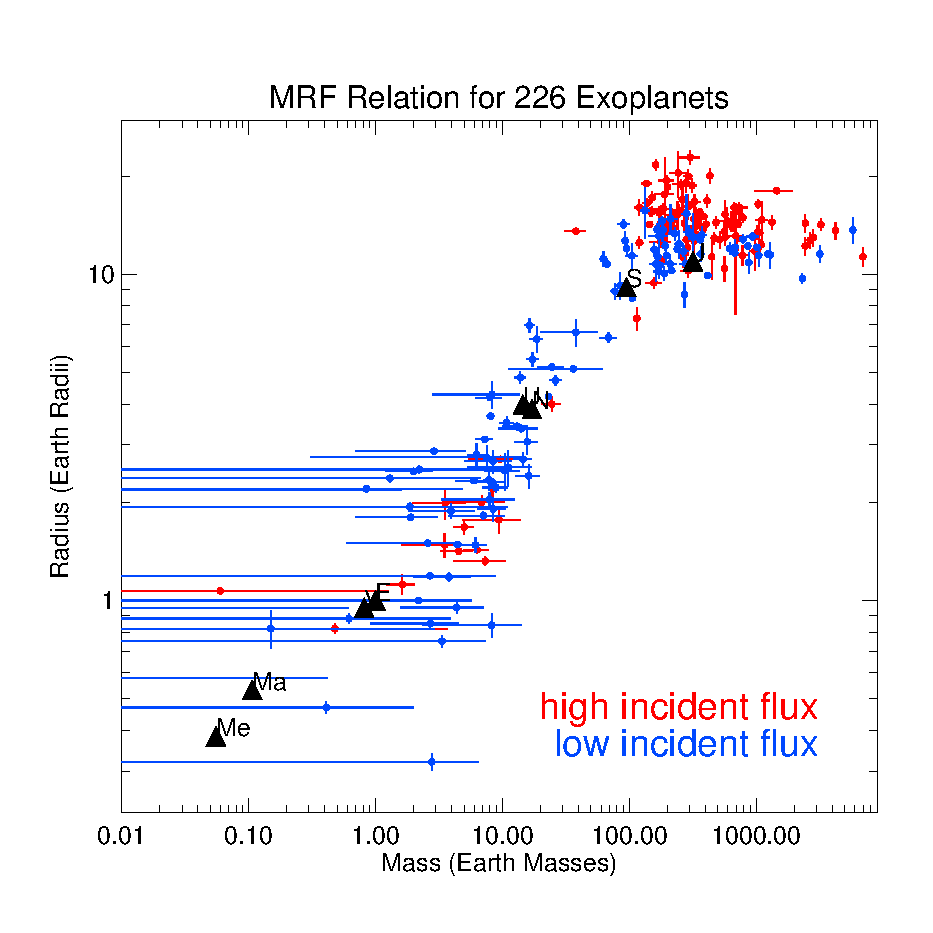
\includegraphics[width=6in]{mrf.eps} 
   \caption{Radius vs. mass for exoplanets with measured masses and radii.  Planets receiving lower than the median incident flux from this sample (459 times the incident flux at Earth) are blue; those receiving higher than the median incident flux are red.  The Solar System planets are over plotted as black triangles for comparison.  For giant planets ($\mpl \geq \frac{1}{2} M_{\mathrm{Sat}}$), planet radius correlates with incident flux, whereas for the smaller planets, radius and incident flux appear anti-correlated (see Figure \ref{fig:flux_radius}).}
   \label{fig:mrf}
\end{figure}

\begin{figure}[htbp] %  figure placement: here, top, bottom, or page
   \centering
    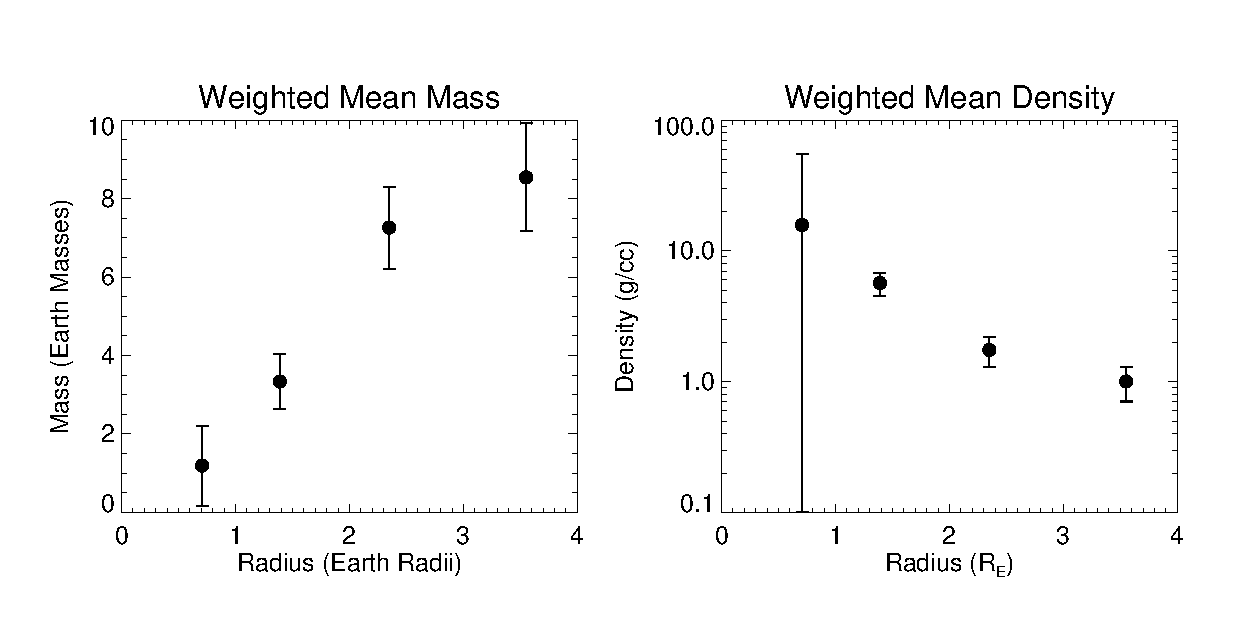
\includegraphics[width=6in]{mr_bin.eps} 
   \caption{The weighted mean mass (left) and density (right) for exoplanets with $\rpl < \rspecial$ in bins of 1 \rearth.  The error bars are the weighted uncertainties in the means.  Larger exoplanet radii correlate with larger masses but lower densities, indicating that large planets have a larger mass fraction of volatiles than small planets.}
   \label{fig:rbin}
\end{figure}

\begin{figure}[htbp] %  figure placement: here, top, bottom, or page
   \centering
    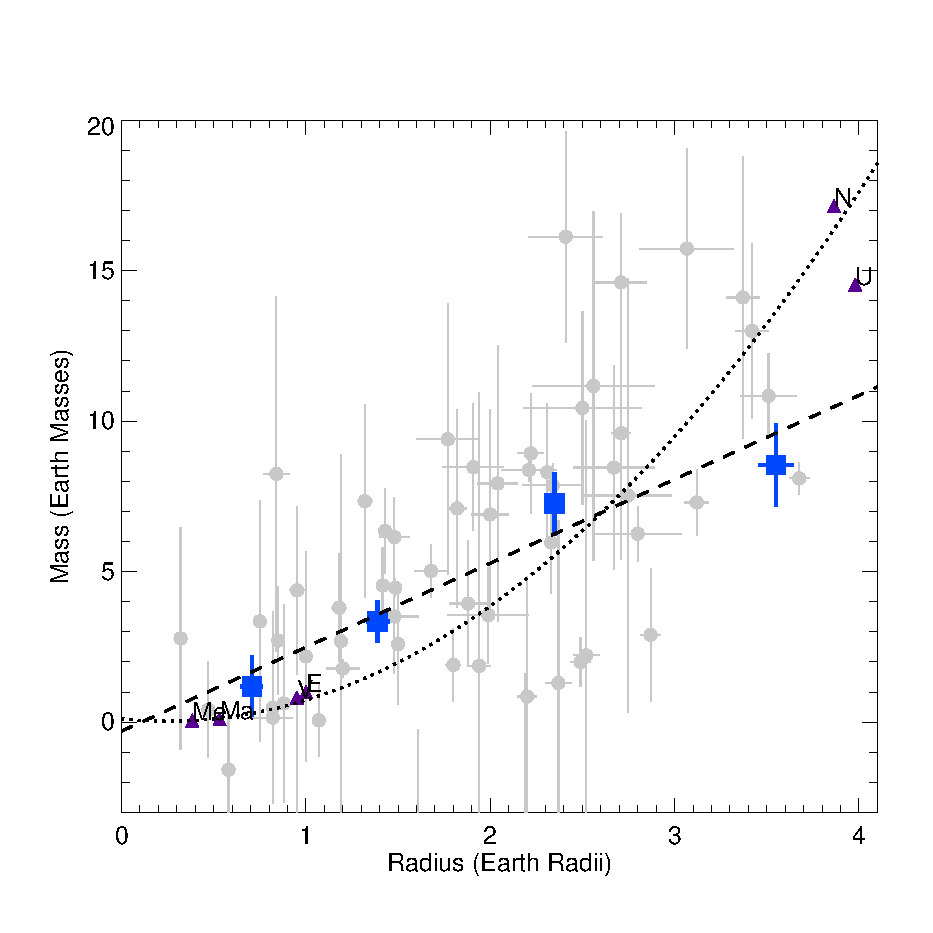
\includegraphics[width=6in]{rm_small4.eps} 
   \caption{Mass vs. radius for 59 planets with $\rpl < 4 \rearth$ and 1$\sigma$ uncertainties.  The dashed line is the best linear fit to the 59 exoplanets: $\mpl/\mearth = 0.2 + 2.6 \times \rpl/\rearth$, $\chi^2/\nu = \chisquared$.  The dotted line is the best quadratic fit to the 59 exoplanets and 6 Solar System planets: $\mpl = 0.1 - 0.6 \rpl + 1.25 \rpl^2$, in which we assumed errors in \mpl and \rpl for S.S. planets were $10^{-5}$ of their values.  Red squares represent the weighted mean mass in bins of 1 \rearth, and error bars are the uncertainty in the mean mass (as in Figure \ref{fig:rbin}), to guide the eye.  Note that a linear fit goes through the the weighted mean of the exoplanet population).  The solar system planets are plotted as blue triangles.  Note that Uranus and Neptune are much colder than the exoplanets in this sample.}
   \label{fig:rm_4}
\end{figure}

\begin{figure}[htbp] %  figure placement: here, top, bottom, or page
   \centering
    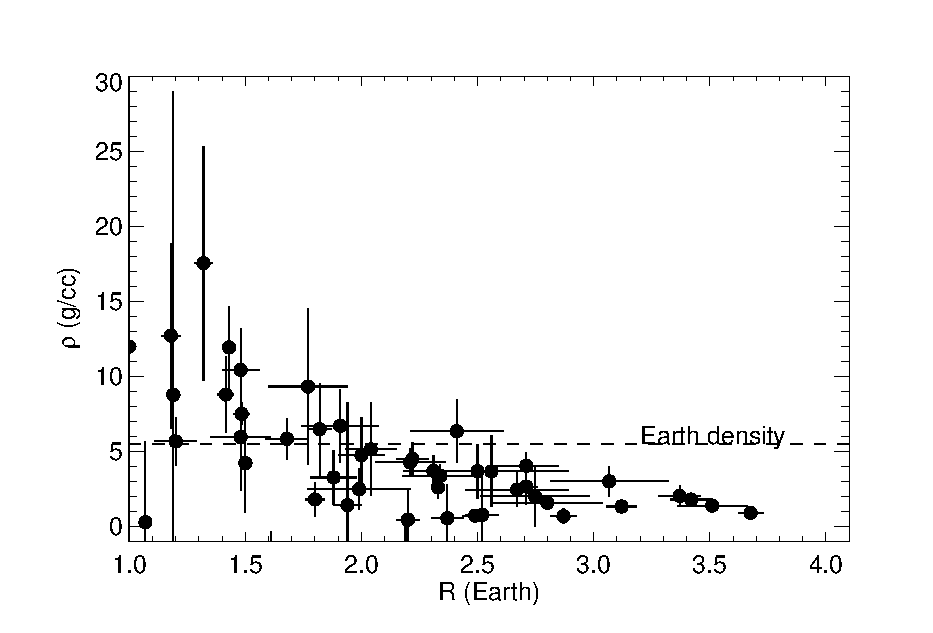
\includegraphics[width=6in]{rhor_4.eps} 
   \caption{Density vs. radius for planets with $\rpl < \rspecial $ and $1\sigma$ uncertainties.  Smaller planets are denser than larger planets.  For reference, the density of Earth (5.5 \gcc) is shown as a dashed line.}
   \label{fig:rhor}
\end{figure}


\begin{figure}[htbp] %  figure placement: here, top, bottom, or page
   \centering
      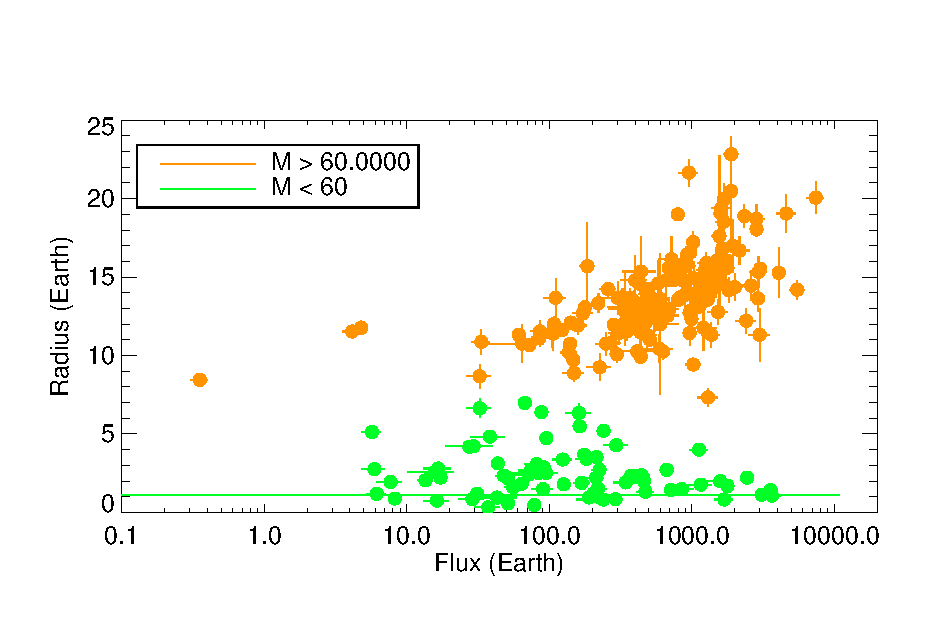
\includegraphics[width=6in]{flux_dependence.eps} 
   \caption{Radius vs. flux and $1\sigma$ uncertainties for exoplanets with measured masses and radii.  Giant planets are orange; low-mass planets are green.  For giant planets, radius increases with increasing incident flux from the star; for small planets, radius slightly decreases with increasing flux, especially above a few hundred Earth fluxes.  There are no hot Neptunes.  Note that all the planets with $\rpl < 4 \rearth$ are in the low-mass population.}
   \label{fig:flux_radius}
\end{figure}


\begin{comment}
\begin{figure}[htbp] %  figure placement: here, top, bottom, or page
   \centering
    \includegraphics[width=6in]{mr_residuals.eps} 
   \caption{Mass residuals (measured minus predicted mass) vs. radius for planets with $\rpl  < \rspecial$ and 1$\sigma$ uncertainties.  The correlation between mass residuals and orbital parameters is too small to be significant.}
   \label{fig:resids}
\end{figure}
\end{comment}

%%%%%%%%%%%%% Discussion %%%%%%%%%%%%%%%%%%%%%%%%%%%%%%%%
\clearpage

\bibliography{exoplanet_papers}{}
\bibliographystyle{apj}

\end{document}  